\section{Proactor}
\label{sec:proactor}

The Proactor architectural pattern allows event-driven applications to efficiently demultiplex and dispatch service requests triggered by the completion of asynchronous operations, to achieve the performance benefits of concurrency without incurring certain of its liabilities.


\subsection*{Context}

An event-driven application that receives and processes multiple service requests asynchronously.


\subsection*{Problem}

By processing multiple requests asynchronously, the performance of event-driven applications, such as servers, can often be increased. To support asynchonous operations, the application must be able to react to completion events of the async operations, which are delivered by the operating system. Typically four aspects need to be taken into account:

\begin{itemize}
	\item For scalability and low latency, multiple completion events should be processed simultaneously
	\item To maximize throughput, unnecessary context switching should be avoided.
	\item Extending the set of available services should require minimal effort.
	\item Application code should largely be shielded from the threading and synchronization mechanisms.
\end{itemize}


\subsection*{Solution}

Split each application service into long-duration operations and completion handlers. Long-duration operations are executed asynchronously and the completion handlers processes the result of these operations as they finish. Further, decouple dispatcher and completion event demultiplexing from the application-specific processing (so the application specific code only has to provide a long-duration async operation and a completion handler).


\subsection*{Structure}

\begin{itemize}
	\item \emph{handle}: provided by operating systems to identify entities which can generate completion events (i.e. for a file or socket)
	\item \emph{asynchonous operation}: application specific, async operation
	\item \emph{completion handler}: application specific handler for completion of asynchronous operation
	\item \emph{concrete completion handler}: the actual implementation of a completion handler
	\item \emph{asynchonous operation processor}: executes async operations and queues completion events (often implemented by and OS kernel)
	\item \emph{completion event queue}: filled with completion events on async operation completion
	\item \emph{asynchronous event demultiplexer}: removes and returns a completion event (can block)
	\item \emph{proactor}: calls demultiplexer, demultiplexes \& dispatches to completion handler. Provides an event loop for the application.
	\item \emph{initiator}: i.e. accepts incoming connections, and invokes async operation. Part of the application. Often also plays the role of a concrete completion handler to be able to process the result of the operation it invoked.
\end{itemize}


\subsection*{Implementation}

Two layers:
\begin{itemize}
	\item Demultiplexing/dispatching infrastructure layer components: Performs generic, application-indipendent logic to execute async operations and demultiplexes and dispatches completion events.
	\item Application layer components: Defines application specific asynchronous operations and completion handlers
\end{itemize}

\begin{figure}[H]
	\centering
	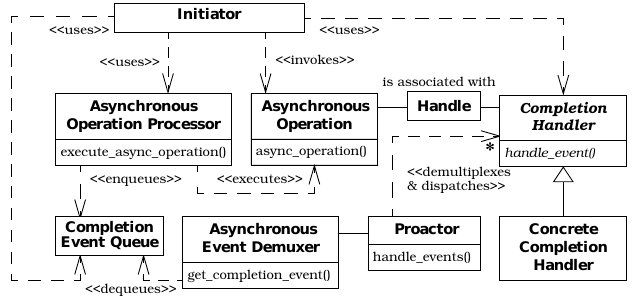
\includegraphics[width=12cm]{content/posa2/proactor/images/uml-diagram.jpeg}
	\caption{proactor uml diagram}
\end{figure}


\subsection*{Varianten}
\begin{itemize}
	\item \emph{Asynchronous Completion Handlers}\\
	Completion handlers act as initiators, so they can also perform long-duration async operations.
	\item \emph{Concurrent Asynchronous Event Demultiplexer}\\
	Maintain a pool of threads to which the proactor can demultiplex and dispatch completion handlers concurrently.
	\item \emph{Shared Completion Handlers}\\
	Multiple async operations can share the same completion handler. Proactor and Initiator must collaborate in this case to know which opertaion requires which completion handler.
	\item \emph{Asynchronous Operation Processor Emulation}\\
	Some programming environments do not export async operations to applications (i.e. the JVM). In such cases async operations can be emulated using a concurrency mechanism.
\end{itemize}


\subsection*{Known uses}

\begin{itemize}
	\item Completion ports in Windows NT: OS is the async operation processor and provides the completion event queue with the complection ports.
	\item POSIX AIO family of async I/O: Similar to Windows NT, but preemitvely async (completion can interrupt thread)
	\item ACE Proactor Framework
	\item OS device driver interrupt-handling mechanisms
	\item Phone call initiation via voice mail
\end{itemize}


\subsection*{Benefits}

\begin{itemize}
	\item Separation of Concerns
	\item Portability by abstracting the async operation mechanisms and using the proactor to shield the application from non-portable completion event demultiplexing and dispatching mechanisms.
	\item Encapsulation of concurrency mechanisms
	\item Decoupling of threading from concurrency
	\item Performance
	\item Simplification of application synchronization
\end{itemize}


\subsection*{Liabilities}

\begin{itemize}
	\item Restricted applicability
	\item Complexity of programming, debugging and testing
	\item Scheduling, controlling, and canceling asynchronously running operations
\end{itemize}
